%%
%% Automatically generated ptex2tex (extended LaTeX) file
%% from Doconce source
%% http://code.google.com/p/doconce/
%%




%-------------------------- begin preamble --------------------------
\documentclass[twoside]{article}



\usepackage{relsize,epsfig,makeidx,amsmath,amsfonts}
\usepackage[latin1]{inputenc}
\usepackage{minted} % packages needed for verbatim environments


% Hyperlinks in PDF:
\usepackage[%
    colorlinks=true,
    linkcolor=black,
    %linkcolor=blue,
    citecolor=black,
    filecolor=black,
    %filecolor=blue,
    urlcolor=black,
    pdfmenubar=true,
    pdftoolbar=true,
    urlcolor=black,
    %urlcolor=blue,
    bookmarksdepth=3   % Uncomment (and tweak) for PDF bookmarks with more levels than the TOC
            ]{hyperref}
%\hyperbaseurl{}   % hyperlinks are relative to this root

% Tricks for having figures close to where they are defined:
% 1. define less restrictive rules for where to put figures
\setcounter{topnumber}{2}
\setcounter{bottomnumber}{2}
\setcounter{totalnumber}{4}
\renewcommand{\topfraction}{0.85}
\renewcommand{\bottomfraction}{0.85}
\renewcommand{\textfraction}{0.15}
\renewcommand{\floatpagefraction}{0.7}
% 2. ensure all figures are flushed before next section
\usepackage[section]{placeins}
% 3. enable begin{figure}[H] (often leads to ugly pagebreaks)
%\usepackage{float}\restylefloat{figure}

\newcommand{\inlinecomment}[2]{  ({\bf #1}: \emph{#2})  }
%\newcommand{\inlinecomment}[2]{}  % turn off inline comments

% insert custom LaTeX commands...

\makeindex

\begin{document}
%-------------------------- end preamble --------------------------





% ----------------- title -------------------------

\begin{center}
{\LARGE\bf Effects of Hill Shapes \\ [1.5mm] on Tsunami Simulations}
\end{center}




% ----------------- author(s) -------------------------

\begin{center}
{\bf Kristian Pedersen and Gustav Baardsen} \\ [0mm]
%{\bf Hans Petter Langtangen${}^{1, 2}$ (\texttt{hpl@simula.no})} \\ [0mm]
\end{center}

%\begin{center}
% List of all institutions:
%\centerline{{\small ${}^1$Center for Biomedical Computing, Simula Research Laboratory}}
%\centerline{{\small ${}^2$Department of Informatics, University of Oslo.}}
%\end{center}
% ----------------- end author(s) -------------------------



% ----------------- date -------------------------


\begin{center}
\today
\end{center}

\vspace{1cm}



\begin{abstract}

In this project we study how the shape of hills at the sea bottom
affects numerical and physical properties of simulations of
 earthquake-generated tsunamis. The tsunamis are modelled using 
two-dimensional wave equations, and a finite difference scheme is 
used to solve the partial differential equations.


\end{abstract}

\tableofcontents



% Section with multi-line equation.
\section{Introduction}

\label{Introduction}
In this text we will address a two-dimensional, standard linear wave equation, with damping and reflecting boundaries. We will develop a scheme for solving it and apply it to the problem of a tsunami over an uneven seabed. Especial focus will be put on the question of which kinds of seabeds causes numerical instability. 

\section{Mathematical model}

\label{Model}
For $(x, y)$ in the domain $D = [0,L_y] \times [0,L_x]$ and $t \in [0,T]$, we will study the partial differential equation
\begin{equation}
u_{tt} + b u_{t} = (q(x, y)u_{x})_{x} + (q(x, y)u_{y})_{y} + f(x, y, t), 
\end{equation}
where $(x, y) \in D$ and $t \in [0, T]$, with the boundary and initial conditions
\begin{align}
\frac{\partial u}{\partial n} &= 0 & (x, y) \in \partial D,  t \in [0, T], \nonumber \\
u(x, y, 0) &= I(x, y) &x,y \in \partial D, \nonumber \\
u_{t}(x, y, 0) &= V(x, y) &x,y \in \partial D.
\end{align} 
Here $\partial D$ denotes the boundary of the domain $D$ and $\partial /\partial n$ stands for differentiation in the normal direction out of the boundary.

\section{Numerical scheme}

\label{Scheme}
\subsection{Numerical scheme for the inner points}
In operator notation, we want to use the following scheme for inner points:
\begin{align}
[D_{t} D_{t} u + b D_{2t} u = D_{x}(q D_{x} u) + D_{y} (q D_{y} u) +f]_{i\, j}^{n} \label{PDE}
\end{align}
Calculating each summand we find:

\begin{align}
[D_{t} D_{t} u]_{i\, j}^{n} &= \frac{u^{n+1}_{i, j} - 2u^{n}_{i, j} + u^{n-1}_{i, j}}{\Delta t^{2}} \label{Dttu}, \\
[bD_{2}t u]_{i\, j}^n &= b\frac{u^{n+1}_{i,j} - u^{n-1}_{i,j}}{2\Delta t} \label{bD2tu}, \\
[D_x q D_x u]_{i\, j}^n &= \frac{q_{i +\frac{1}{2},j}(u^{n}_{i+1,j} - u^{n}_{i,j}) - q_{i -\frac{1}{2},j}(u^{n}_{i,j} - u^{n}_{i-1,j})}{\Delta x^2} \label{DxqDxu}, \\
[D_y q D_y u]_{i\, j}^n &= \frac{q_{i,j +\frac{1}{2}}(u^{n}_{i,j+1} - u^{n}_{i,j}) - q_{i ,j-\frac{1}{2}}(u^{n}_{i,j} - u^{n}_{i,j-1})}{\Delta x^2} \label{DyqDyu}, \\
[f]_{i\, j}^n &= f(x_i, y_{j}, t_{n}). \label{f}
\end{align}
Inserting these expressions into Eq. (\ref{PDE}) and solving for $u^{n+1}_{i,j}$, we get the following scheme for inner points:
\begin{align}
u^{n+1}_{i,j} &= \left\{ 2u^{n}_{i,j} + u^{n-1}_{i,j} \right. \nonumber \\
& \left. + \frac{\Delta t^2}{\Delta x^2}\left(q_{i +\frac{1}{2},j}(u^{n}_{i+1,j} - u^{n}_{i,j}) - q_{i -\frac{1}{2},j}(u^{n}_{i,j} - u^{n}_{i-1,j})\right) \right. \nonumber \\ 
&\left. +  \frac{\Delta t^2}{\Delta y^2} \left(q_{i,j +\frac{1}{2}}(u^{n}_{i,j+1} - u^{n}_{i,j}) - q_{i ,j-\frac{1}{2}}(u^{n}_{i,j} - u^{n}_{i,j-1})\right) \right. \nonumber \\
&\left. + \Delta t^{2} f(x_i, y_j, t_n) \right\}/\left( 1 + \frac{1}{2}b\Delta t \right)
\end{align}

\subsection{Numerical scheme for the first time step}
For the first time step $n = 0$, $u^{n-1}_{i,j}$ is not a part of the grid. To circumvent this problem, we have to apply the intial condition $u_t(x,y,0) = V(x,y) \text{ for } x,y \in \partial D$. We discretize it and get:
$$[D_{2t} u = V]_{i\,j}^0 \implies \frac{u_{i\,j}^1 - u_{i\,j}^{-1}}{2\Delta t} = V(x_i,y_j) \implies u_{i\,j}^{-1} = u_{i\,j}^{1} - 2\Delta t V(x_i,y_j).$$
Inserting this into equation (\ref{Dttu}) and (\ref{bD2tu}), we get:
\begin{align}
[D_t D_t u]_{i\, j}^n &= 2\left(\frac{u^{n+1}_{i,j} - u^{n}_{i,j}}{\Delta t^2}  - \frac{V(x_i,y_i)}{\Delta t}\right), \\
[bD_{2t} u]_{i\, j}^n &= b\frac{V(x_i,y_i)}{\Delta t}. \label{bD2tu2}
\end{align}
Inserting these expressions into Eq. (\ref{PDE}) and solving for $u^{n+1}_{i,j}$, we get the following scheme for inner points in the first time step $n = 0$:
\begin{align}
u^{n+1}_{i,j} &= u^{n}_{i,j} + \left( 1 - \frac{1}{2}b\Delta t\right)\Delta t V_{i,j} \nonumber \\
&+ \frac{\Delta t^2}{2\Delta x^2} \left( q_{i +\frac{1}{2},j}(u^{n}_{i+1,j} - u^{n}_{i,j}) - q_{i -\frac{1}{2},j}(u^{n}_{i,j} - u^{n}_{i-1,j})\right) \nonumber \\ 
&+  \frac{\Delta t^2}{2\Delta y^2} \left( q_{i,j +\frac{1}{2}}(u^{n}_{i,j+1} - u^{n}_{i,j}) - q_{i ,j-\frac{1}{2}}(u^{n}_{i,j} - u^{n}_{i,j-1})\right) \nonumber \\
 &+ \frac{\Delta t^2}{2} f(x_{i}, y_{j}, t_{n}).
\end{align}


\subsection{Numerical scheme for the boundary}
On the boundary, this scheme needs points outside the defined space domain. For example, we need values for $u_{-1, j}^{n}$, $u_{i, N_{y}+1}^{n}$, and $u_{0, -1}^{n}$.
Values for these points can be obtained from the discretized versions of the Neumann condition. The Neumann conditions are in discretized form
\begin{align}
[D_{2x} u]_{0\, j}^n = [D_{2x} u]_{N_{x}\, j}^n = 0 & \quad \text{ for } j = 0, 1,\ldots , N_{y}, \quad n = 0, 1, \dots , N_{t}, \\
[D_{2y} u]_{i\, 0}^n = [D_{2y} u]_{0,N_{y}}^n = 0 & \quad \text{ for } i = 0, 1, \dots , N_y, \quad n = 0, 1, \dots , N_{t},
\end{align}
which leads to the equations
\begin{align}
u_{1,j}^n = u_{-1,j}^n ,  \quad u_{N_x-1,j}^n = u_{Nx+1,j}^n  & \quad \text{ for } j = 0, 1, \ldots , N_{y}, \quad n = 0, 1, \ldots , N_{t} \\
u_{i,1}^n = u_{i,-1}^n, \quad u_{i,Ny+1}^n = u_{i,Nx+1}^n & \quad \text{ for } i = 0, 1, \ldots , N_{y},\quad n = 0, 1, \ldots , N_{t}.
\end{align}
A scheme for the borders can now be found by applying each equality to the inner point scheme for its boundary. The corners are found by applying two equalities, one for each of the adjecent border.

\subsection{Approximating q(x,y) outside the grid}

In our implementation, we assume that values for the function $q(x, y)$ are given only at the grid points $(x_{i}, y_{j})$. In the finite difference algorithm, we use mean values to evaluate the function at other points. To approximate the $q$ function when evaluated outside the grid, we will apply the arithmetic and harmonic mean, defined respectively as
\begin{align}
  q_{i+\frac{1}{2},j} &= \frac{q_{i,j} + q_{i+1,j}}{2} \label{armean} \\
\end{align}
and
\begin{align}
  q_{i+\frac{1}{2},j} &= 2 \left(\frac{1}{q_{i,j}} + \frac{1}{q_{i+1,j}}\right)^{-1}. \label{harmean}
\end{align}
When not states explicitly otherwise, we have used the arithmetic mean as the default option.


\section{Implementation}

We implemented the code in pure python. See the wave2D\_du0.py for the full code.

TODO: Show the core of the program in minted enviroment


%% The numerical method is implemented in a Python function:

%% \begin{minted}[fontsize=\fontsize{9pt}{9pt},linenos=false,mathescape,baselinestretch=1.0,fontfamily=tt,xleftmargin=7mm]{python}
%% def theta_rule(I, a, T, dt, theta):
%%     """Solve u'=-a*u, u(0)=I, for t in (0,T] with steps of dt."""
%%     N = int(round(T/float(dt)))  # no of intervals
%%     u = zeros(N+1)
%%     t = linspace(0, T, N+1)

%%     u[0] = I
%%     for n in range(0, N):
%%         u[n+1] = (1 - (1-theta)*a*dt)/(1 + theta*dt*a)*u[n]
%%     return u, t
%% \end{minted}

% Section with figures.


\section{Numerical experiments}

%\index{numerical experiments}

\subsection{Verification}

The implementation of the finite difference algorithm was verified with the following tests:  

\begin{itemize}
\item In the first test the initial conditions were set to 
  \begin{align}
    u(x, y, t=0) & \equiv I(x, y) = u_{0}, \nonumber \\
    u_{t}(x, y, t=0) & \equiv V(x, y) = 0,
  \end{align}

  where $u_{0}$ is a constant, and we used the restriction $f(x, y, t) = 0$. The resulting PDE gives the constant solution $u(x, y, t) = u_{0}$.
\item In the second test case, the 2-dimensional code was tested with the simple one-dimensional plug function 
  \begin{displaymath}
  I(x, y) = \left\{ \begin{array}{ll}
    0 & \text{ if } |x - L/2| > a, \\
    1 & \text{ else, }
  \end{array} \right.
\end{displaymath}

as initial condition. In the case with $V(x, y) = 0$, $f(x, y, t) = 0$, and
$q(x, y) = c^{2}$, where $c$ is a constant, the solution $u(x, y, t)$ gives
exactly two moving squares, as long as the Carnot number $C \equiv c\Delta t/ \Delta x$ is 1. This test was repeated by interchanging $x$ and $y$ in the initial condition.

\item As another one-dimensional test, we used the one-dimensional initial conditions
  \begin{align}
    I(x, y) & = \exp\left(a(x - L/2)^{2}\right), \nonumber \\
    V(x, y) & = 0,  
  \end{align}
where $a$ is a constant, togehter with the restrictions $b = 0$ and $f(x, y, t) = 0$. These conditions give the solution
\begin{align}
  u(x, y, t) &= \frac{1}{2}\exp\left(-a(x-ct-L_{x}/2)^{2}\right) \nonumber \\
  & = + \frac{1}{2}\exp\left(-a(x + ct - L_{x}/2\right)^{2}),  
\end{align} 
at the limit when the boundaries are infinitely far away. This solution does not fulfill the boundary condition $\partial u/\partial n = 0$, but it was a useful test for the first few steps of the simulation.

\item As suggested in the project description, we also used the manufactured solution 
  \begin{equation}
    u(x, y, t) = \exp\left( -bt\right)\cos\left( \omega t\right)\cos\left( \frac{m_{x}x\pi }{L_{x}}\right)\cos\left( \frac{m_{y}y\pi }{L_{y}}\right),
  \end{equation}
where $b$ is the damping parameter in the studied PDE, $\omega $ is a real constant, and $m_{x}$ and $m_{y}$ are integers. The solution $u(x, y, t)$ is a standing wave with the desired boundary condition $\partial u/\partial n = 0$. This manufactured solution was tested both with constant $q$ and with the choise $q(x, y) = \exp(-x-y)$. For both cases we had to determine functions $f(x, y, t)$ such that the given manufactured solution fulfills the two-dimensional wave equation.
According to the project formulation, the error $\varepsilon $ of the solution $u(x, y, t)$ should converge as  
\begin{equation}
  \varepsilon = Dh^{2},
\end{equation}
where
\begin{equation}
  D = D_{t}F_{t}^{2}+D_{x}F_{x}^{2}+D_{y}F_{y}^{2},
\end{equation}
$\Delta t = F_{t}h $, $\Delta x = F_{x}h$, $\Delta y = F_{y}h$, and $D_{i}$ and $F_{i}$, $i \in \{ t, x, y \}$, are constants.

In our implementation, the convergence rate $r$ was estimated by assuming the relation between rates of subsequent errors $\varepsilon_{k}$ with decreasing parameter $h_{k}$ and rates of the convergence parameter $h_{k}$ being of the form
\begin{equation}
  \frac{\varepsilon_{h_{k-1}}}{\varepsilon_{h_{k}}} = \left(\frac{h_{k-1}}{h_{k}}\right)^{r}.
\end{equation}
Here the considered error was chosen to be 
\begin{equation}
  \varepsilon_{h_{k}} = \max_{i, j} \left|u_{e}(x_{i}, y_{j}, t_{N})-u_{h_{k} i,j}^{N}\right|,
\end{equation}
where $u_{e}(x, y, t)$ is the exact solution and $u_{h_{k} i,j}^{N}$ is the numerical solution with convergence parameter $h_{k}$. Examples of calculated convergence rates are given in Table \ref{tab:conv}.

\end{itemize}

  \begin{table} \label{tab:conv}
    \begin{center}
      \caption{Convergence rates $r_{k}$ for different convergence parameters $h_{k}$ and two different choises of the function $q(x, y)$.}
      \begin{tabular}{ccc}
        \hline\hline
        $h_{k}$ & $q = $ const. & $q(x, y) = \exp(-x-y)$ \\
        \hline
        0.01 & 1.959 & 1.984 \\
        0.001 & 1.996 & 1.998 \\
        \hline\hline

      \end{tabular}
    \end{center}
  \end{table}

  \subsection{One-dimensional simulations}
  
  We did some simulations with one-dimensional systems to get a better view of 
  the behaviour of the solutions. With the one-dimensional systems, it was also possible to use finer mesh grids. In the directories \verb+movie_1dwave_box_Ba250+ and \verb+movie_1dwave_gaussian_Bs250+ we have examples of simulations of one-dimensional systems with a box and a Gaussian shaped hill, respectively. With the same hight of the hill, the simulation with a Gaussian perturbation gave a smoother function $u(x, y, t)$ than what was the case with the box-shaped perturbation.  

\begin{figure} 
  \centering
  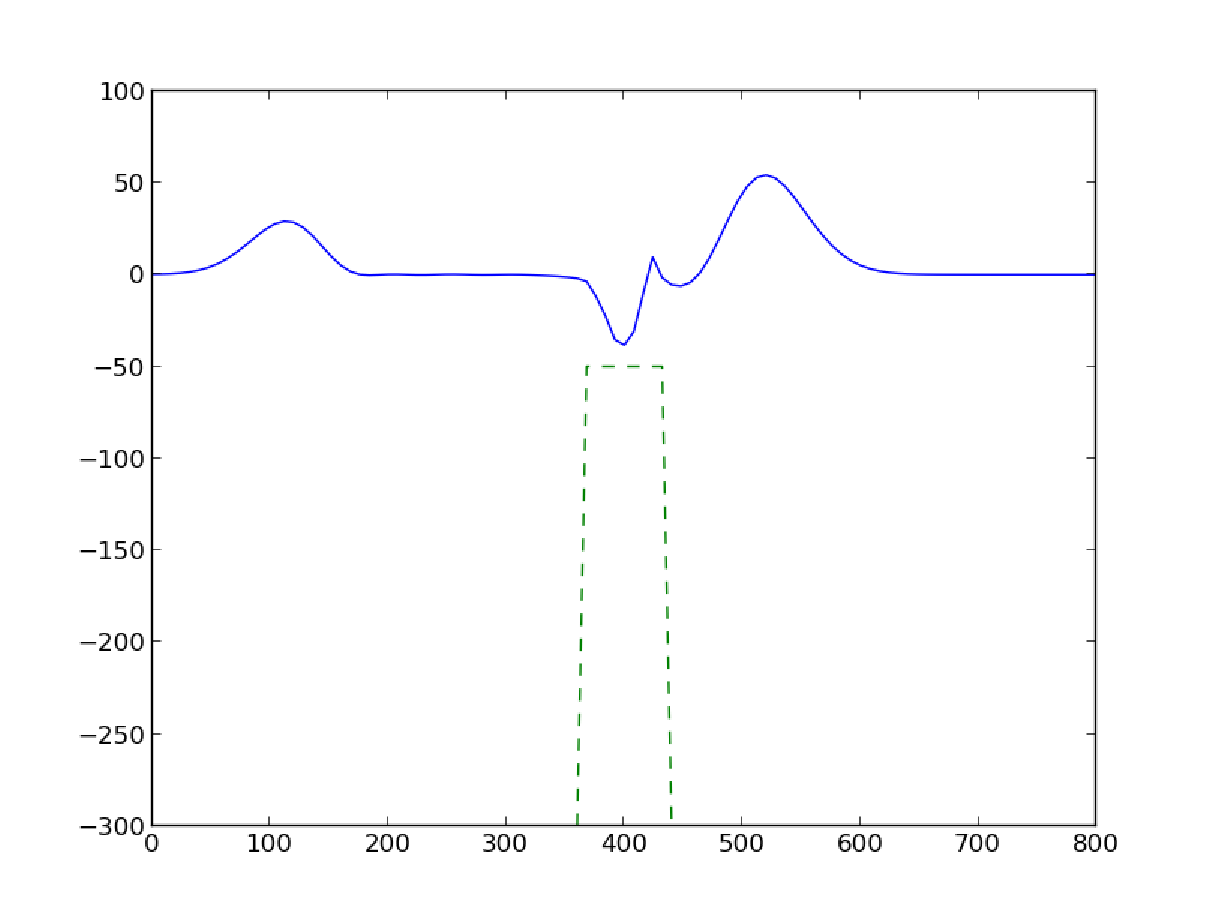
\includegraphics[scale=0.4]{gustavs_codes/movie_1dwave_box_Ba250/figure.pdf}
  \caption{A snapshot of a one-dimensional simulation with a box-shaped hill at the bottom of the sea. The solution is clearly not smooth, and has probably numerical noise.} %\label{fig:}
\end{figure}

\begin{figure} 
  \centering
  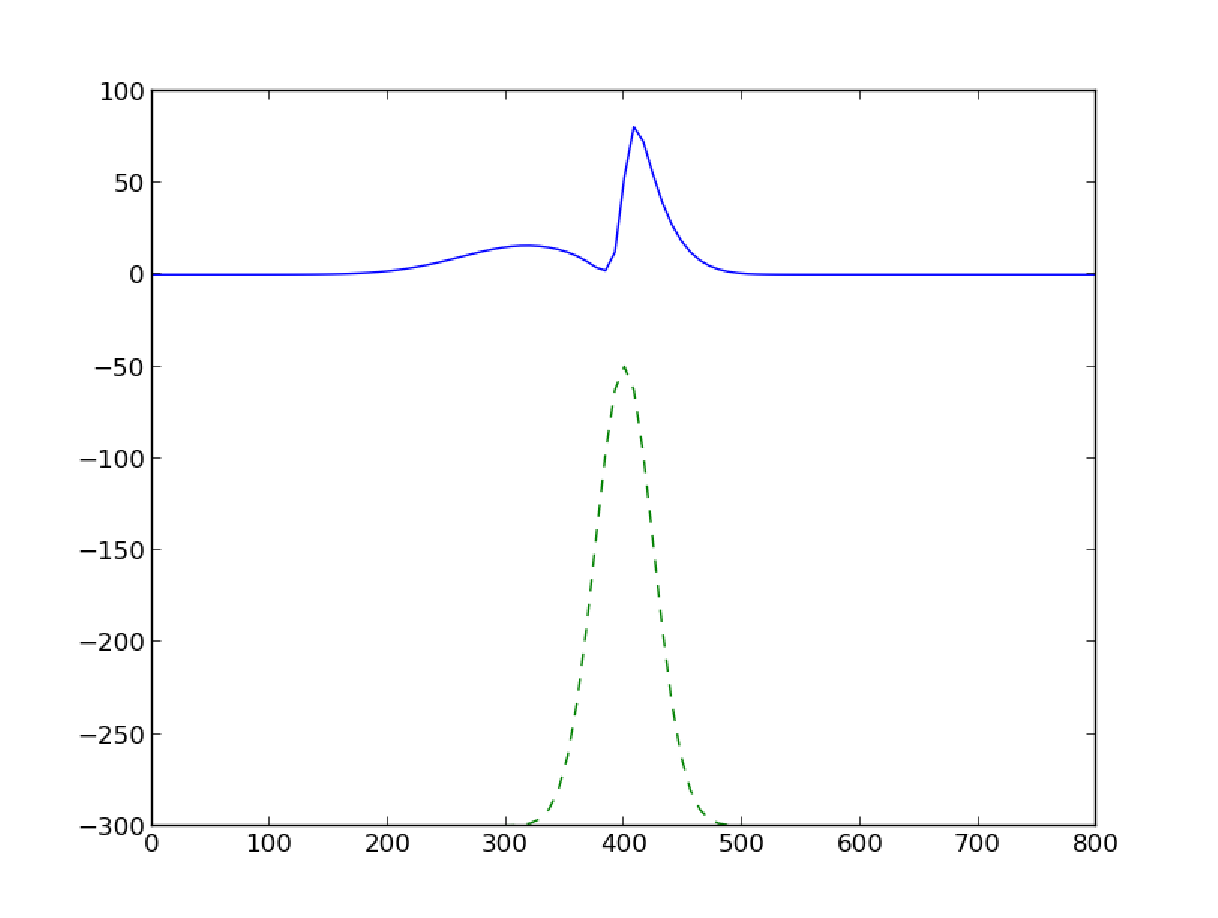
\includegraphics[scale=0.4]{gustavs_codes/movie_1dwave_gaussian_Bs250/figure.pdf}
  \caption{A picture from a one-dimensional simulation with a Gaussian-shaped hill at the seabed. This solution is smoohter than the result of the simulation with a box-sahped hill, but is partially quite sharp.} %\label{fig:}
\end{figure}

Even if the solution of the Gaussian case is partially sharp, the numerical result becomes quite smooth when adding more space grid points. In the directories \verb+movie_1dwave_gaussian_Bs275_Nx100+ and \newline \verb+movie_1dwave_gaussian_Bs275_Nx200+, there are simulation results obtained with the same Gaussian perturbation, whence the number of space grid points was 100 and 200 in the two runs, respectively. From these movies one clearly sees that the numerical solution becomes smooth when using a finer space mesh.

We also did a comparison between two simulations with the same box perturbation and 100 versus 200 mesh grid points. As in the case with a Gaussian hill, the numerical solution improved with a finer mesh. However, it seems that the system with a box hill may have a solution that is not smooth for any number of space mesh points. It is difficult to say, based on these simulations, what is numerical noise and what is due to a mathematically oscillating or non-smooth function. A first step in investigating that could be to compare numbers for $u_{i,\ j}^{n}$ of simulations with different numbers of grid points, using large $N_{x}$. It would perhaps also be instructive to look for exact numerical solutions for simple cases with a discontinuous $q$ function. 
 
Another question we asked was how the width of the box hill affects the quality of the numerical solution. A snap-shot from a simulation is shown in Fig. \ref{fig:box_1d_narrow}, and the movie is stored in the directory \verb+movie_1dwave_box_Ba275_Bs15_Nx200+. At least, the solution is more spectacular with a narrower box perturbation. Still, it is not possible to say whether this is due to numerical noise or an oscillating shape of the exact solution. Intuitively, it is plausible that a geometry with sharp forms gives rise to high-frequency components, which in turn may lead to sharp and/or oscillating solutions. Generally, we observed that there were very clear reflections of part of the wave at the discontinouity points of the $q$ function. When using smoother hills, the reflections became more spread out.

\begin{figure} 
  \centering
  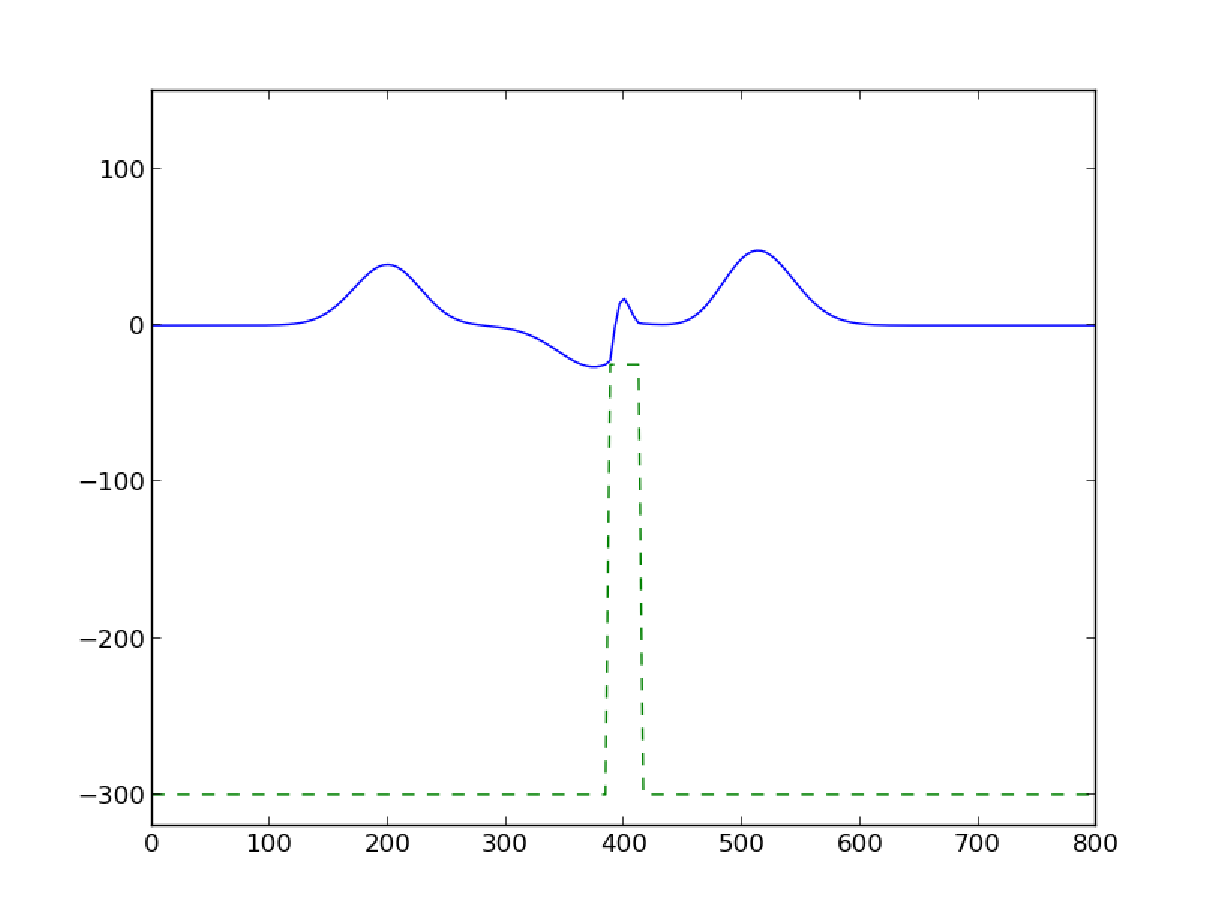
\includegraphics[scale=0.4]{gustavs_codes/movie_1dwave_box_Ba275_Bs15_Nx200/figure.pdf}
  \caption{An example from a simulation with a narrow box hill. The resulting function is more spectacular than what was obtained with a wider box.} \label{fig:box_1d_narrow}
\end{figure}

The latter observation was studied closer using discontinuous and smooth step functions. The smooth step function was of the form 
\begin{equation}
  B(x, y) = B_{0} + \frac{B_{a}}{1 + \exp\left(-(x-B_{mx})/B_{s}\right)}, 
\end{equation}
where $B_{0}$, $B_{a}$, $B_{mx}$, and $B_{s}$ are parameters. These geometries might be used to simulate a tsunami approching a shore where the sea level decreases suddenly. The related movies are stored in the directories \verb+movie_1dwave_box_shore+ and \newline \verb+movie_1dwave_smooth_step+. We found that the reflected wave was sharper peaked in the case with a discontinuous step function, whereas the smooth step function gave a reflected wave more smeared out. However, both simulations had similar sharp oscillations behind the main wave. This oscillation may be a numerical artefact. One can also observe how the wave moves slower on the shallower water. This is natural, as the function $q(x, y)$ is proportional to both the depth of the sea, $B(x, y)$, and the squared of the wave velocity, $c^{2}$. From a physical point of view, the wave uses energy to keep the wave pulse higher, and therefore has less energy left for moving horisontally.

\begin{figure} 
  \centering
  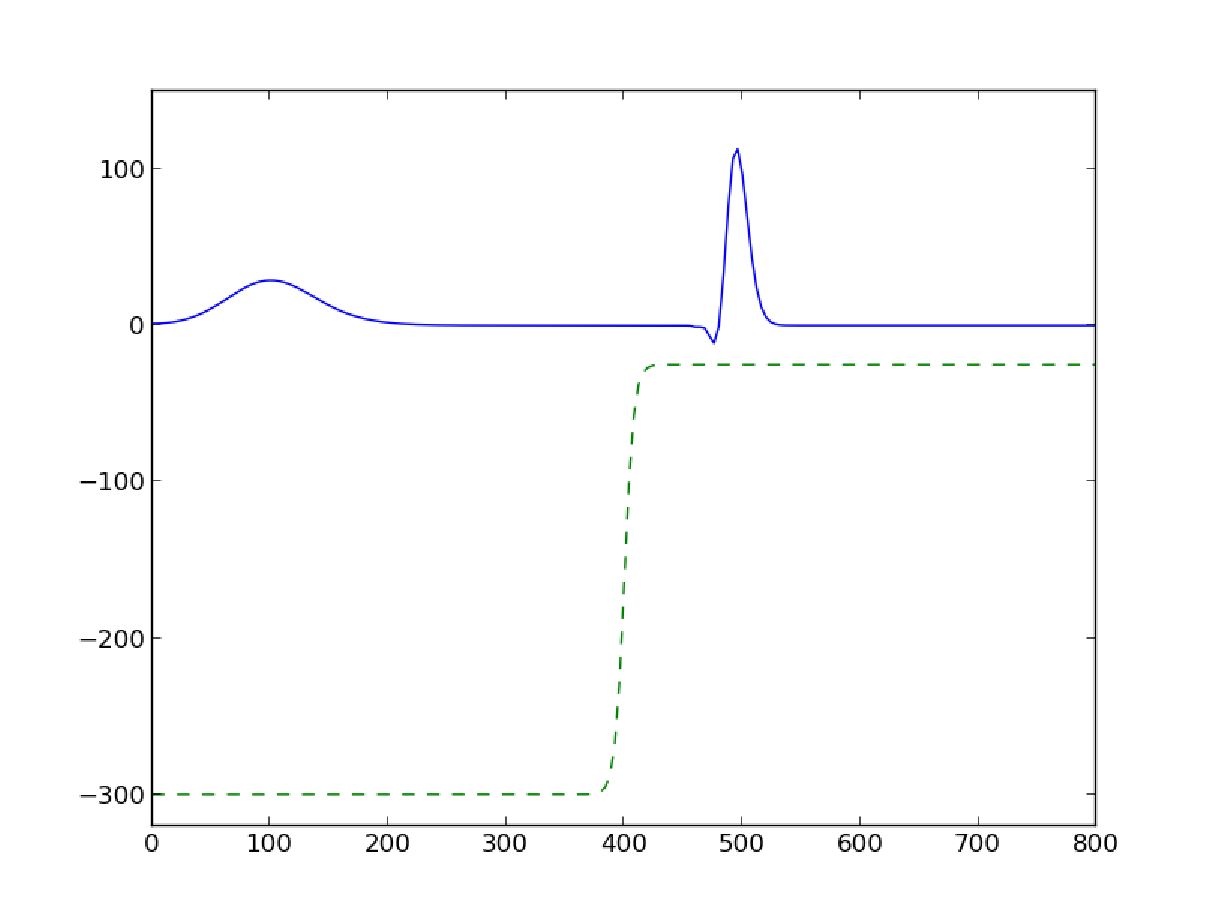
\includegraphics[scale=0.4]{gustavs_codes/movie_1dwave_smooth_step/figure.pdf}
  \caption{A smooth step function is used at the shore. The reflected wave pulse is more smeared out than in the case with a sharp step function. This result shows oscillations behind the main pulse, which may be numerical noise.}
\end{figure}

\begin{figure} 
  \centering
  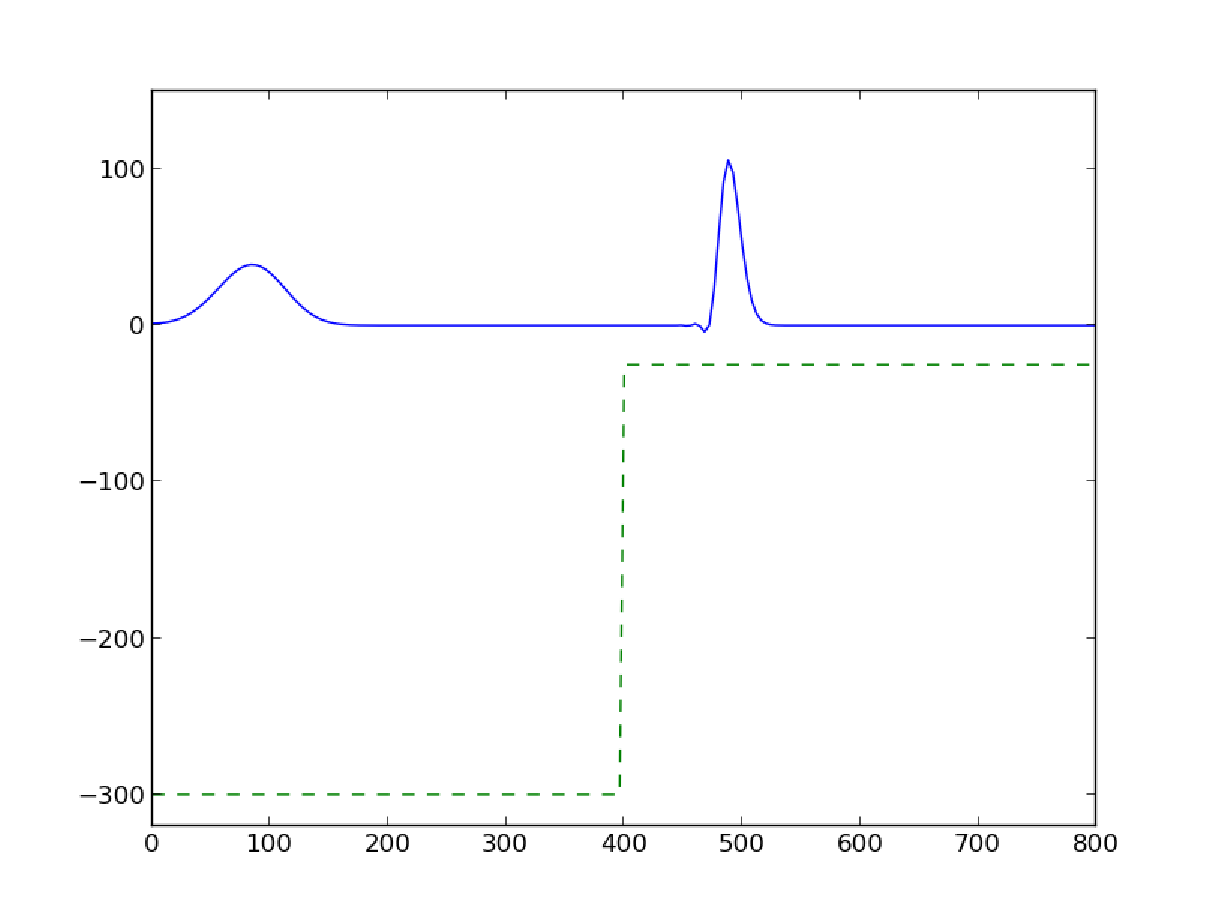
\includegraphics[scale=0.4]{gustavs_codes/movie_1dwave_box_shore/figure.pdf}
  \caption{The shore is modelled using a sharp step function. In this case the reflected wave is sharp. As in the case with a smoother step function, here is also seen oscillations behind the main wave pulse.}
\end{figure}
 

\section{Conclusions}

%\begin{figure}[!ht]
%  \centerline{\includegraphics[width=0.9\linewidth]{error.png}}
%  \caption{
%  Error versus time step. \label{fig:E}
%  }
%\end{figure}
%\clearpage % flush figures fig:E

\printindex

\end{document}
